\documentclass[18pt]{beamer}
\usepackage{templates/beamerthemekit}
\usepackage[export]{adjustbox}
\usepackage{tikz}
\usepackage{url}
\usepackage{marvosym} % \MVRIGHTarrow
\usepackage{stmaryrd} % \shortrightarrow
\usepackage{textcomp} % \textrightarrow
\usepackage{svg}

\title[Short Project-Plan]{Towards Bringing Together Numerical Methods for Differential Equation and Deep Neural Networks}
\subtitle{Short Project-Plan,  Supervisor - Markus Hoffmann}
\author{Stanislav Arnaudov}
\institute{Chair for Computer Architecture and Parallel Processing}
\selectlanguage{english}

% \usepackage[style=verbose,backend=bibtex]{biblatex}
% \bibliography{bib}
% \bibliographystyle{plain}

\begin{document} 

\begin{frame}
 \titlepage
\end{frame}


\section{Motivation}
\begin{frame}
  \frametitle{Motivation}
  \begin{columns}
    \begin{column}{0.5\textwidth}
      \large{\underline{Differential equation (DEs)}}
      \begin{itemize}
      \item used in simulations
      \item hard to solve numerically
      \item solutions have image representation
      \end{itemize}
      \vspace{0.25cm}
      \textbf{Goal}: solve DEs based on their image representation
      \vspace{-0.5cm}
    \end{column}
    \begin{column}{0.5\textwidth}
      \begin{center}
        \begin{figure}[htb]
          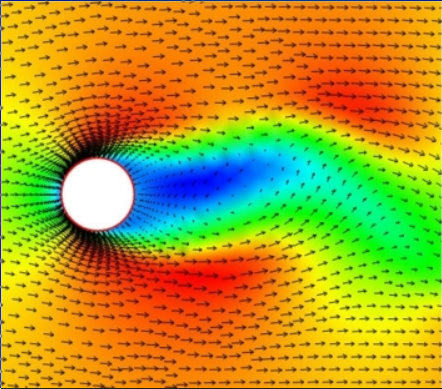
\includegraphics[scale=0.35]{images/pde}
          \caption{Flow Simulation\footnotemark}
        \end{figure}
      \end{center}
    \end{column}
    \footnotetext{``Team for Advanced Flow Simulation and Modeling'', Professor Tayfun E. Tezduyar, Sunil Sathe}
  \end{columns}
\end{frame}

\section{Question and Topic}
\begin{frame}
  \frametitle{Research topic and research question}
  \large{\underline{Research topic:}}\\
  \vspace*{0.2cm}
  The relationship between differential equations and neural networks.
  \vspace*{2cm}
  \\
  \large{\underline{Research question:}}
  \vspace*{0.2cm}
  \\
  How can we develop a deep neural network that can solve time dependent differential equations based on the image representation of their solutions?
\end{frame}

\section{System and planning}
\begin{frame}[t]
  \frametitle{Project}
  \begin{center}
    \large{\underline{Simulation:}}
  \end{center}
  \begin{figure}[htb]
    \includesvg[scale=0.7]{images/new/sim_1}
  \end{figure}
  \vspace{2cm}  
  \begin{itemize}
  \item Sequence of time steps.
  \item Information about time step is to be generated.
  \end{itemize}  
\end{frame}

\begin{frame}[t]
  \frametitle{Project}
  \begin{center}
    \large{\underline{Simulation:}}
  \end{center}
  \begin{figure}[htb]
    \includesvg[scale=0.7]{images/new/sim_2}
  \end{figure}
  \vspace{2cm}  
  \begin{itemize}
  \item Sequence of time steps.
  \item Differential equation for each time step.
  \end{itemize}  
\end{frame}

\begin{frame}[t]
  \frametitle{Project}
  \begin{center}
    \large{\underline{Simulation:}}
  \end{center}
  \begin{figure}[htb]
    \includesvg[scale=0.7]{images/new/num_system}
  \end{figure}
  \vspace{0.7cm}  
  \begin{itemize}
  \item The DE are usually solved with a numerical solver.
  \end{itemize}  
\end{frame}

\begin{frame}[t]
  \frametitle{Project}
  \begin{center}
    \large{\underline{Simulation:}}
  \end{center}
  \begin{figure}[htb]
    \includesvg[scale=0.6]{images/new/nn_system}
  \end{figure}
  \vspace{0.3cm}  
  \begin{itemize}
  \item We take advantage of the image representation of the solutions.
  \end{itemize}  
\end{frame}

\begin{frame}[t]
  \frametitle{Numerical solver\slash Generating data}
    \begin{columns}
      \begin{column}{0.5\textwidth}
        \begin{figure}[htb]
          \includesvg[scale=0.6]{images/new/num}
        \end{figure}
        \begin{figure}[htb]
          \centering
          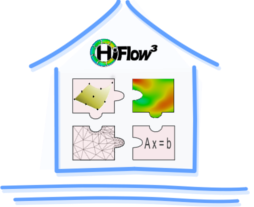
\includegraphics[scale=0.7]{images/new/hiflow_house}
        \end{figure}
      \end{column}
      \begin{column}{0.5\textwidth}
        \large{\underline{HiFlow:}}
        \begin{itemize}
        \item framework for solving DE
        \end{itemize}
        \vspace{2cm}
        \large{\underline{Tasks:}}
        \begin{itemize}
        \item generate training data for the network
        \item solve the first time step of the simulation
        \end{itemize}        
      \end{column}
  \end{columns}
\end{frame}



\begin{frame}[t]
  \frametitle{Network}
    \begin{columns}[t]
      \begin{column}{0.5\textwidth}
        \begin{figure}
          \centering
          \includesvg[scale=0.6]{images/new/nn}
        \end{figure}
        
      \end{column}
      \begin{column}{0.5\textwidth}
        \large{\underline{Network:}}
        \begin{itemize}
        \item image as an input
        \item image as an output
        \end{itemize}
        \vspace{2cm}
        \large{\underline{Tasks:}}
        \begin{itemize}
        \item find an appropriate architecture
        \item implement in Python
        \item fine-tune hyper-parameters of the network
        \end{itemize}
      \end{column}
  \end{columns}
\end{frame}


\begin{frame}[t]
  \frametitle{Training}
  \begin{columns}[t]
    \begin{column}{0.5\textwidth}
      \begin{figure}[htb]
        \centering
        \includesvg[scale=0.6]{images/new/nn_train}
      \end{figure}
      
    \end{column}
    \begin{column}{0.5\textwidth}
      \large{\underline{Loss function:}}
      \begin{itemize}
      \item appropriately compare images in our context
      \end{itemize}
      \vspace{2cm}
      \large{\underline{Tasks:}}
      \begin{itemize}
      \item find an appropriate loss function
      \item train the network
      \end{itemize}
    \end{column}
  \end{columns}
\end{frame}

\begin{frame}[t]
  \frametitle{Evaluating}
  \begin{columns}[t]
    \begin{column}{0.5\textwidth}
      \begin{figure}[htb]
        \centering
        \includesvg[scale=0.6]{images/new/nn_test}
      \end{figure}
    \end{column}
    \begin{column}{0.5\textwidth}
      \vspace{3.2cm}

      \large{\underline{Tasks:}}
      \begin{itemize}
      \item apply the network to different simulations
      \item investigative the error when the network is applied repeatedly
      \end{itemize}
      
    \end{column}
  \end{columns}
\end{frame}

\begin{frame}
  \frametitle{}
  \begin{center}
    \huge{Thank you for your attention.}    
  \end{center}
\end{frame}

\begin{frame}
  \frametitle{}
  \begin{center}
    \huge{Questions?}
  \end{center}
\end{frame}




\end{document}

%%% Local Variables:
%%% mode: latex
%%% TeX-master: t
%%% End:
